% Summary index document for the analysis chapter
\chapter{Analyse}
\label{chap:Analyse}

In diesem Kapitel wird unsere Wahl der Programmiersprache und \acs{PCAP}-Library erläutert.

\todo{JAN: Kapitel überarbeiten, Analyse des Problems am Anfang.}

\section{Einführung}
Gemäss der Aufgabenstellung dieser \work ist die Programmiersprache für das \tool frei wählbar mit der einzigen Voraussetzung dass man eine \acs{PCAP}-Library einbinden kann. In der Inception-Phase des Projekts ging es daher darum eine geeignete Sprache und Bibliothek zu wählen.

\section{JNetPcap}
\label{sec:JNetPcap}

todo Jan

\section{Golang und goPacket}
\label{sec:Golang und goPacket}

\subsection{Golang}
Golang, auch Go genannt, ist eine eher junge Programmiersprache seit 2007 von Google Inc. entwickelt wurde. Golang hat einen C-ähnlichen Syntax, bietet aber viele Eigenschaften von modernen Programmiersprachen wie zum Beispiel Garbage Collection, Type-Safety, Dynamic-Typing, Closures und eine grosse Standard-Library.
Im Oktober 2009 wurde die Golang der Öffentlichkeit als Open Source zur Verfügung gestellt.

\subsection{Evaluation}
Unseren ersten Kontakt mit Golang haben wir durch GoProbe von Open Systems gewonnen.
GoProbe erlaubt leichtgewichtiges aggregieren von Paketen und deren effiziente Speicherung. Eine Abfrage der gespeicherten Paketen ist via Querying Flows möglich.


\section{Performance Vergleich}
\label{sec:Performance Vergleich}

\subsection{Testaufbau}
2 Desktop-Rechner der HSR sind via Gigabit-Lan miteinander verbunden. Auf den Rechnern läuft Ubuntu 14.04 x64 sowie jPerf und die jeweils getestete Software.

%todo Grafik mit MS Visio die unser Testaufbau darstellt.

\subsection{Testdurchführung}
Auf einem der beiden Rechnern läuft jeweils jPerf im Server-Modus sowie die getestete Software. Auf dem anderen Computer läuft jPerf im Client-Modus.
Via. jPerf wird nun soviel Traffic erzeugt um die 1Gbit/s-Leitung möglichst stark auszulasten, d.h. durchschnittlich 900mbit/s. Die getestete Software zeichnet dabei die ganzen Pakete auf und sollte dabei 300mbit/s an Traffic ertragen können. 300mbit/s sind gem. Open Systems AG die Lastspitzen mit denen etwa zu rechnen sind.

\subsection{Ergebnisse}
Java und Golang sind von den Ergebnissen her recht ähnlich. Beide haben die Anforderung von 300mbit/s erfolgreich erfüllt. Golang ist mit den Durchschnittlich 17\% CPU Auslastung etwas performanter als Java. Die 31\% CPU Lastspitze bei Java gibt es jeweils nur wenn das Programm zum ersten Mal gestartet wird und kommt daher dass dann die ganze \acs{JVM} zuerst hochgefahren werden muss.
Beim Memory siehts bei goProbe klar besser aus weil es den ganzen \acs{JVM} Overhead nicht hat.

\begin{table}[h]
\begin{tabular}{|l|l|l|l|}
\hline
\rowcolor[HTML]{C0C0C0} 
\textbf{Software} & \textbf{CPU Spitze} & \textbf{CPU Ø} & \textbf{Memory Ø} \\ \hline
JNetPcap auf Java & 31\%                & 20\%           & tbd               \\ \hline
goProbe auf Go    & 18\%                & 17\%           & tbd               \\ \hline
\end{tabular}
\end{table}

\section{Entscheidung}
Open Systems AG würde es bevorzugen wenn wir Golang statt Java einsetzen. Die Ergebnisse des Performance-Tests sprechen ebenfalls für Golang. Und wir haben durchaus auch das Interesse einmal eine neue Programmiersprache zu lernen.
In Anbetracht dessen haben wir uns entschieden das \tool mit Golang zu entwickeln.

\section{ESP Aufbau}
\label{sec:ESP Aufbau}

\noindent Encapsulating Security Payload (ESP) wird bei \ac{IPsec} (VPN) eingesetzt. Es gewährleistet die Vertraulichkeit und Integrität von Paketen und kümmert sich um die Authentisierung. Durch diese Integritätssicherung werden Pakete vor Manipulation geschützt. ESP verschlüsselt, im Unterschied zu Authentication Header (AH), die Nutzdaten. Bei AH werden nur die Integrität und Echtheit sichergestellt.\cite{elektronik_kompendium}

\noindent Der ESP Header wird zwischen dem IP Header und dem darunterliegenden Protokoll eingefügt (Transport Mode), oder es kapselt das ganze IP-Paket (Tunnel Mode).\cite{rfc4303}

\noindent Der Tunnel Mode wird vor allem bei der Verbindung zwischen zwei Netzwerken über eine unsichere Verbindung eingesetzt. Der Modus unterstützt aber prinzipiell alle Arten von VPN-Anwendungen. Bei dieser Verwendung wird das ganze IP-Paket verschlüsselt und in ein neues IP-Paket verpackt. So wird das gesamte Paket durch ESP abgeschirmt und die eigentliche IP-Adresse des Absenders ist nicht mehr ersichtlich. Diese Methode hat natürlich einen gewissen Overhead. Es kommen 8 Byte für den ESP-Header, 16-20 Byte ESP-Trailer und für den neuen IP-Header 20 Byte hinzu.\cite{elektronik_kompendium}

\begin{figure}[H]
    \begin{center}
        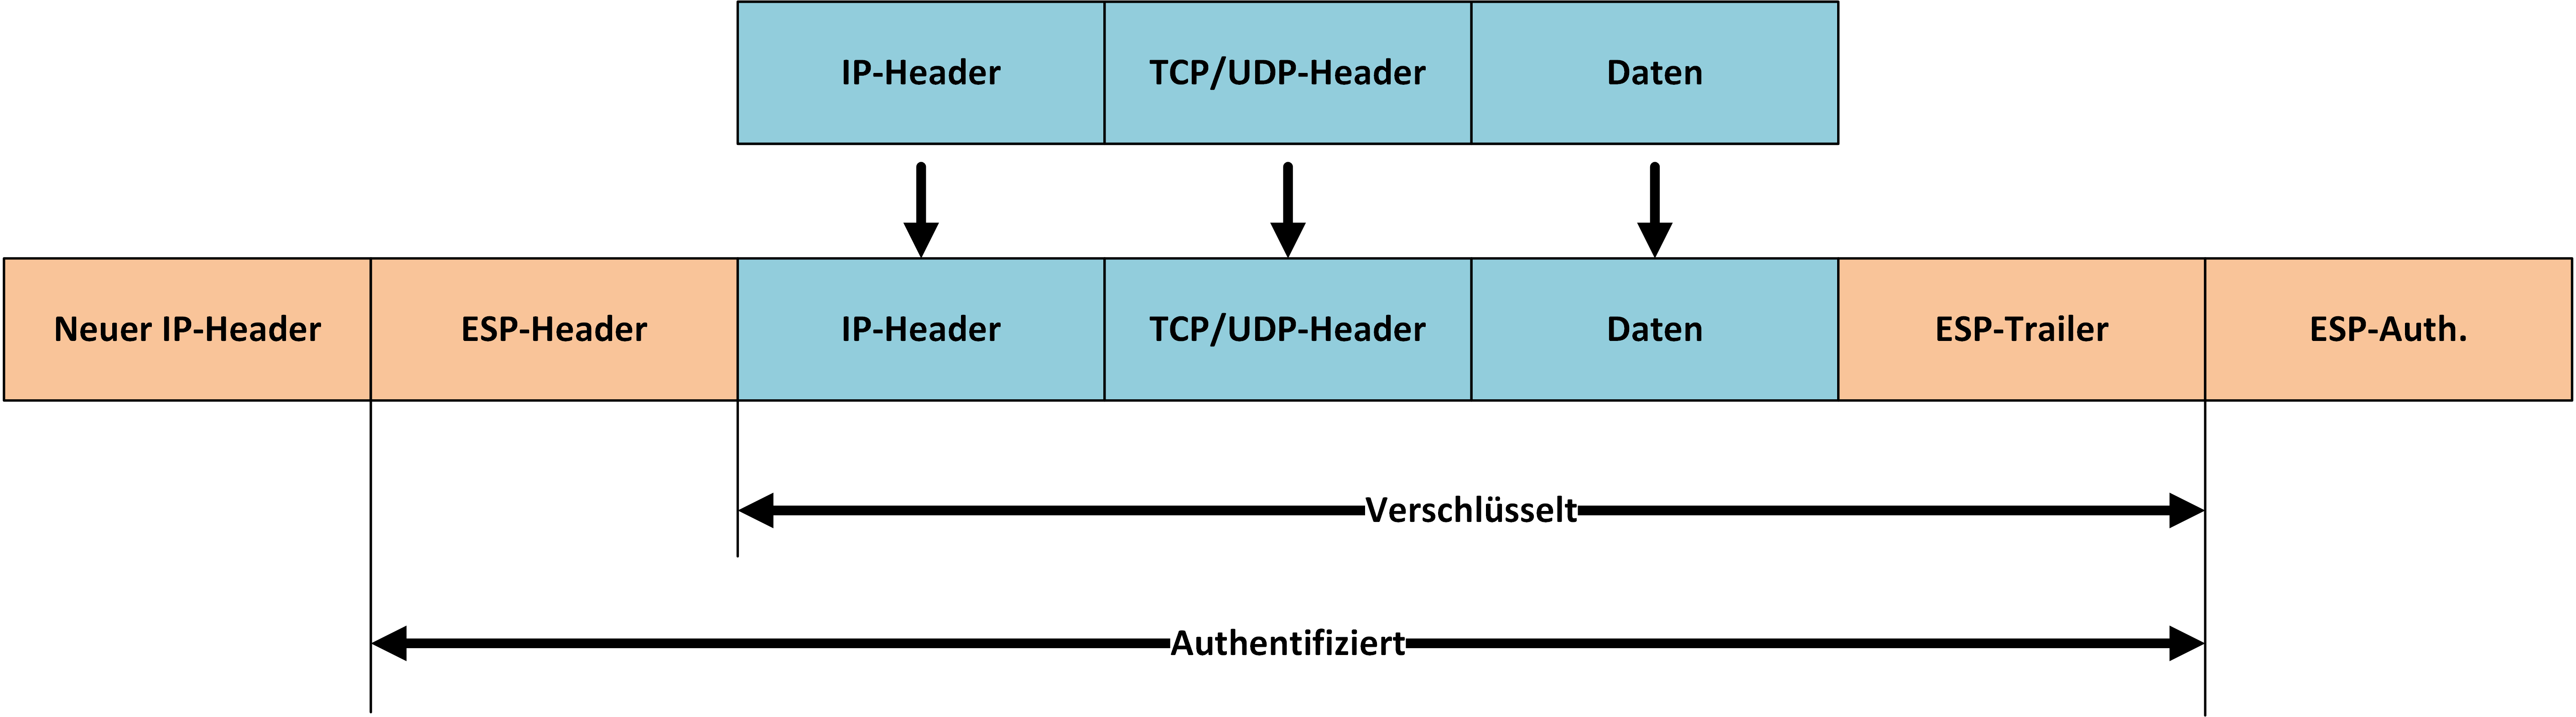
\includegraphics[trim=1 0 0 0,clip,width=\textwidth]{mainpart/analyse/img/ESP_Tunnelmode.png}
    \end{center}
    \caption{Aufbau eines Pakets im Tunnelmode}
\end{figure}

\noindent Bei einer Situation, in der nur zwei Rechner miteinander verbunden werden, kann der Transportmodus verwendet werden. Dieser Modus unterstützt nur Host-to-Host Verbindungen. Da es für \ac{IPsec} nicht unbedingt notwendig ist IP-Pakete vollständig neu zu entkapseln, können beim Transport Mode der originale IP-Header verwendet werden. Es kommen 8 Byte ESP-Header und 16-20Byte ESP-Trailer hinzu. Damit wird der Overhead kleiner, da man keinen zusätzlichen IP-Header benötigt.\cite{elektronik_kompendium}

\begin{figure}[H]
    \begin{center}
        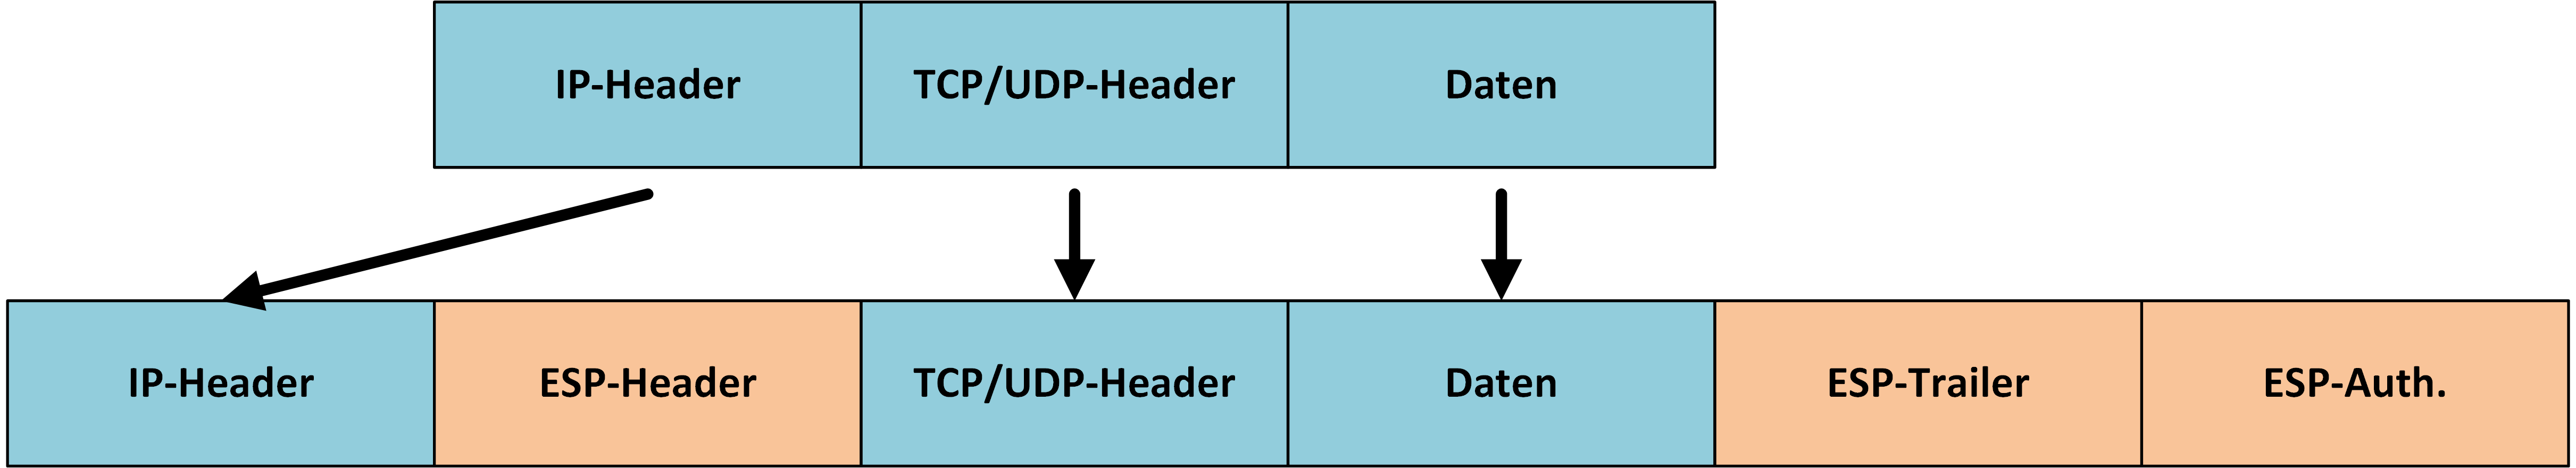
\includegraphics[trim=1 0 0 0,clip,width=\textwidth]{mainpart/analyse/img/ESP_Transportmode.png}
    \end{center}
    \caption{Aufbau eines Pakets im Transportmode}
    %\label{fig:AST_function_call_with_and_without_template_id}
\end{figure}


\textbf{Wichtige Felder}

\begin{table}[H]
\begin{tabularx}{\textwidth}{l|>{\raggedright\arraybackslash}X} 
\hline
Security Parameters\\ Index (SPI) 32bits & Dieser zufällig festgelegte Wert in Kombination mit der IP-Adresse des Ziels wird für eine Identifikation der Verbindung benötigt. Bei jeder neuen Verbindung wird die SPI neu gesetzt.                                                                                                                                                                                                                                                                         \\ \hline
Sequence Number 32bits & Die Sequence Number wird für jedes Paket gesetzt und wird danach für jedes neue Paket um 1 erhöht. Bei einer neuen Verbindung wird die Sequence Number stets auf 1 gesetzt. Falls Anti-Replay eingesetzt wird (standardmässig aktiviert) darf sich die Sequence Number nicht wiederholen. Daher wird, bevor das 2\^{}32 Paket gesendet wird, die Verbindung zurückgesetzt und eine neue SPI ausgehandelt. Damit ist auch die Sequence Number wieder zurückgesetzt. \\
\hline
\end{tabularx}
\caption{Wichtige ESP Felder}
\end{table}

\todo{Jan: Paket Verlust Analyse}

\todo{Theo: MTU Analyse}